%!TeX root=../sensetop.tex
\chapter[Chapter \thechapter]{}
\lettrine[lines=4,lraise=0.3]{M}{rs} Dashwood’s visit to Lady Middleton took place the next day, and two of her daughters went with her; but Marianne excused herself from being of the party, under some trifling pretext of employment; and her mother, who concluded that a promise had been made by Willoughby the night before of calling on her while they were absent, was perfectly satisfied with her remaining at home.

On their return from the park they found Willoughby’s curricle and servant in waiting at the cottage, and Mrs Dashwood was convinced that her conjecture had been just. So far it was all as she had foreseen; but on entering the house she beheld what no foresight had taught her to expect. They were no sooner in the passage than Marianne came hastily out of the parlour apparently in violent affliction, with her handkerchief at her eyes; and without noticing them ran up stairs. Surprised and alarmed they proceeded directly into the room she had just quitted, where they found only Willoughby, who was leaning against the mantel-piece with his back towards them. He turned round on their coming in, and his countenance showed that he strongly partook of the emotion which over-powered Marianne.

\begin{figure}[tbph]
\centering
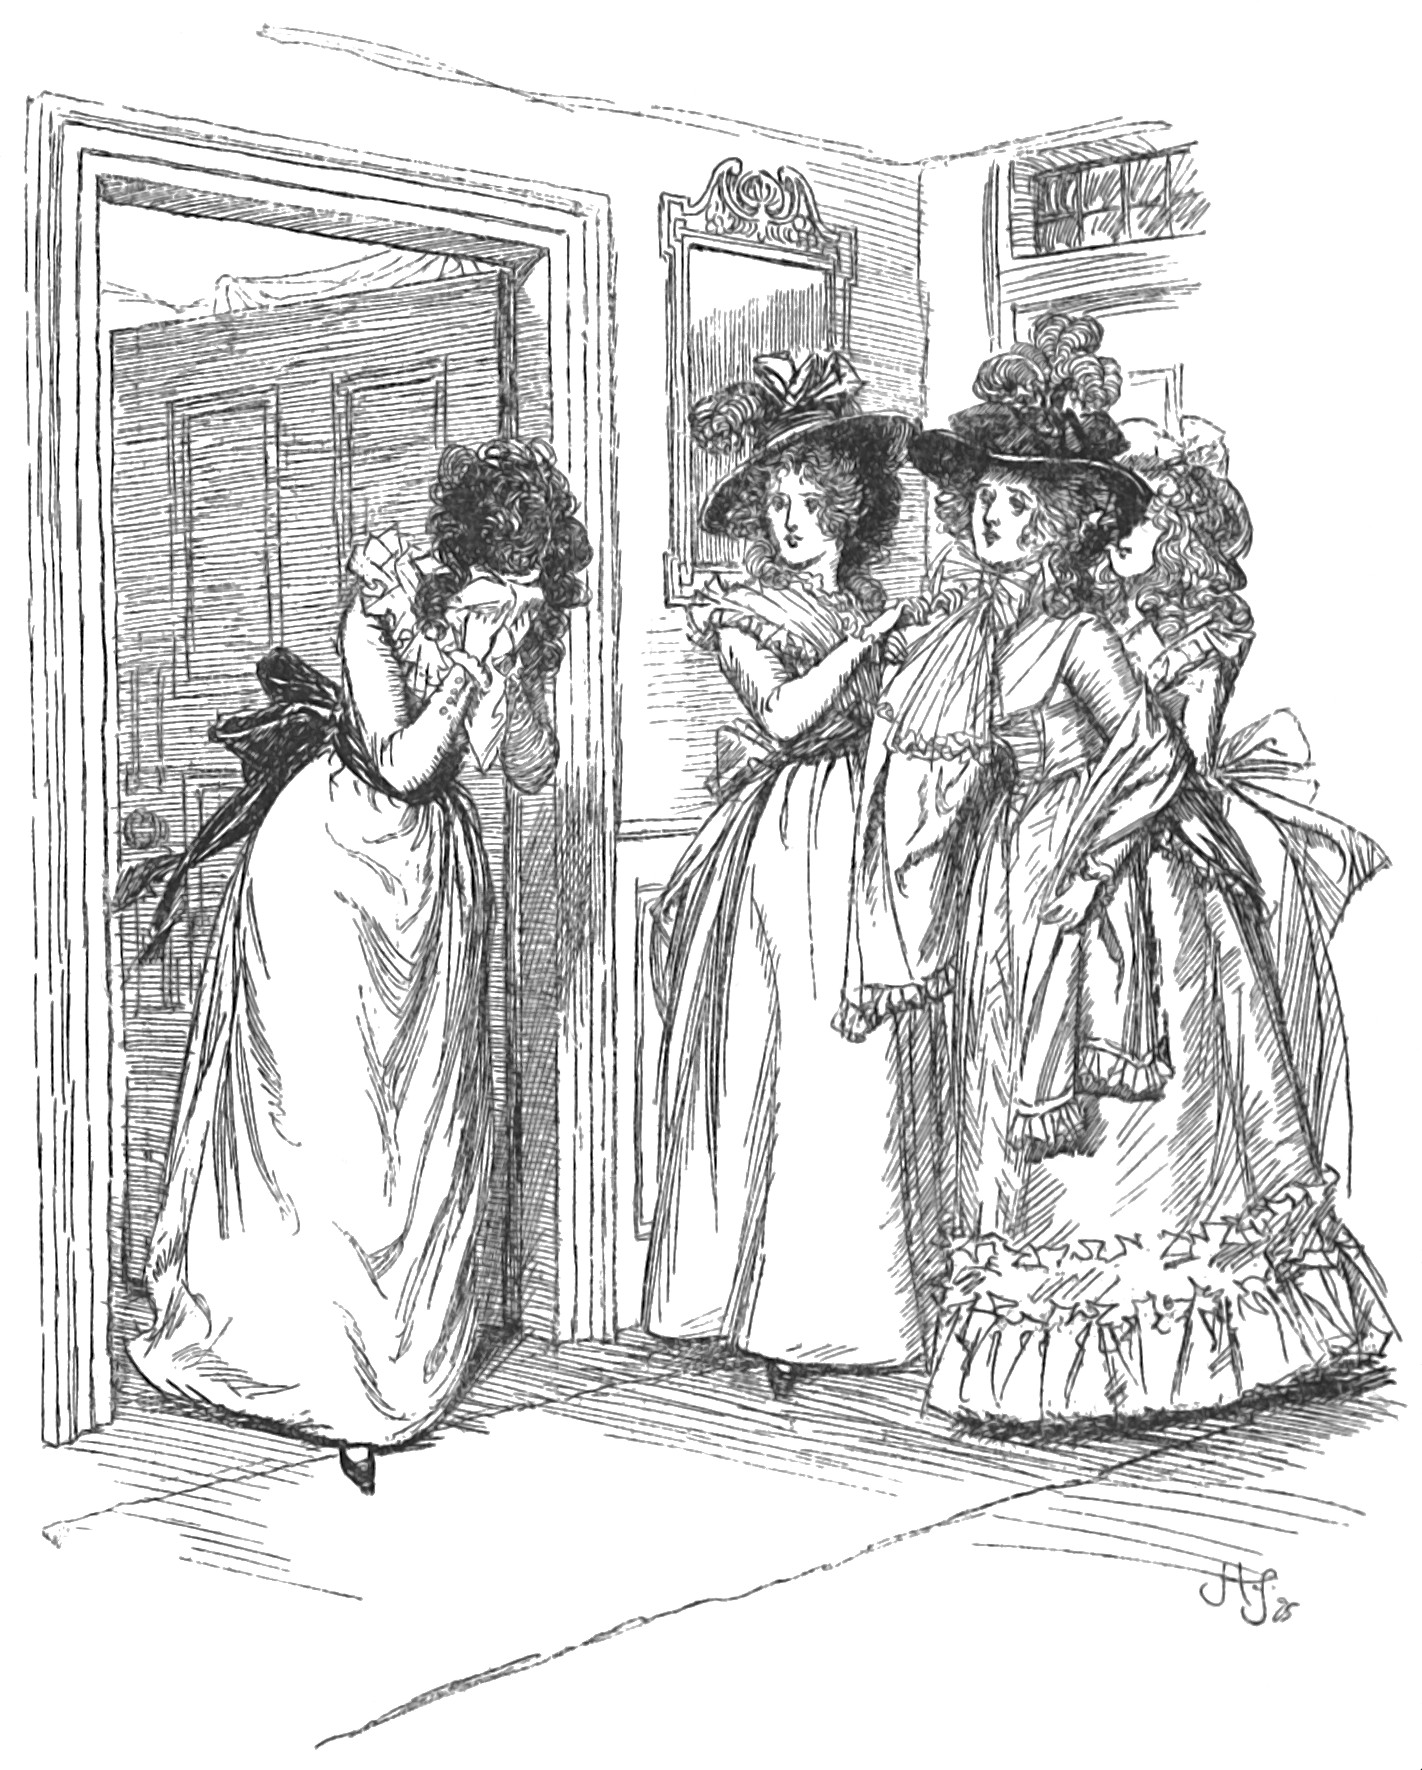
\includegraphics[width=\linewidth]{15affliction}
\caption{Apparently in violent affliction}
\end{figure}

»Is anything the matter with her?« cried Mrs Dashwood as she entered—»is she ill?«

»I hope not,« he replied, trying to look cheerful; and with a forced smile presently added, »It is I who may rather expect to be ill—for I am now suffering under a very heavy disappointment!«

»Disappointment?«

»Yes, for I am unable to keep my engagement with you. Mrs Smith has this morning exercised the privilege of riches upon a poor dependent cousin, by sending me on business to London. I have just received my dispatches, and taken my farewell of Allenham; and by way of exhilaration I am now come to take my farewell of you.«

»To London!—and are you going this morning?«

»Almost this moment.«

»This is very unfortunate. But Mrs Smith must be obliged;—and her business will not detain you from us long I hope.«

He coloured as he replied, »You are very kind, but I have no idea of returning into Devonshire immediately. My visits to Mrs Smith are never repeated within the twelvemonth.«

»And is Mrs Smith your only friend? Is Allenham the only house in the neighbourhood to which you will be welcome? For shame, Willoughby, can you wait for an invitation here?«

His colour increased; and with his eyes fixed on the ground he only replied, »You are too good.«

Mrs Dashwood looked at Elinor with surprise. Elinor felt equal amazement. For a few moments every one was silent. Mrs Dashwood first spoke.

»I have only to add, my dear Willoughby, that at Barton cottage you will always be welcome; for I will not press you to return here immediately, because you only can judge how far \textit{that} might be pleasing to Mrs Smith; and on this head I shall be no more disposed to question your judgment than to doubt your inclination.«

»My engagements at present,« replied Willoughby, confusedly, »are of such a nature—that—I dare not flatter myself\longdash«

He stopped. Mrs Dashwood was too much astonished to speak, and another pause succeeded. This was broken by Willoughby, who said with a faint smile, »It is folly to linger in this manner. I will not torment myself any longer by remaining among friends whose society it is impossible for me now to enjoy.«

He then hastily took leave of them all and left the room. They saw him step into his carriage, and in a minute it was out of sight.

Mrs Dashwood felt too much for speech, and instantly quitted the parlour to give way in solitude to the concern and alarm which this sudden departure occasioned.

Elinor’s uneasiness was at least equal to her mother’s. She thought of what had just passed with anxiety and distrust. Willoughby’s behaviour in taking leave of them, his embarrassment, and affectation of cheerfulness, and, above all, his unwillingness to accept her mother’s invitation, a backwardness so unlike a lover, so unlike himself, greatly disturbed her. One moment she feared that no serious design had ever been formed on his side; and the next that some unfortunate quarrel had taken place between him and her sister;—the distress in which Marianne had quitted the room was such as a serious quarrel could most reasonably account for, though when she considered what Marianne’s love for him was, a quarrel seemed almost impossible.

But whatever might be the particulars of their separation, her sister’s affliction was indubitable; and she thought with the tenderest compassion of that violent sorrow which Marianne was in all probability not merely giving way to as a relief, but feeding and encouraging as a duty.

In about half an hour her mother returned, and though her eyes were red, her countenance was not uncheerful.

»Our dear Willoughby is now some miles from Barton, Elinor,« said she, as she sat down to work, »and with how heavy a heart does he travel?«

»It is all very strange. So suddenly to be gone! It seems but the work of a moment. And last night he was with us so happy, so cheerful, so affectionate? And now, after only ten minutes notice—Gone too without intending to return!—Something more than what he owned to us must have happened. He did not speak, he did not behave like himself. \textit{You} must have seen the difference as well as I. What can it be? Can they have quarrelled? Why else should he have shown such unwillingness to accept your invitation here?«

»It was not inclination that he wanted, Elinor; I could plainly see \textit{that}. He had not the power of accepting it. I have thought it all over I assure you, and I can perfectly account for every thing that at first seemed strange to me as well as to you.«

»Can you, indeed!«

»Yes. I have explained it to myself in the most satisfactory way;—but you, Elinor, who love to doubt where you can—it will not satisfy \textit{you}, I know; but you shall not talk \textit{me} out of my trust in it. I am persuaded that Mrs Smith suspects his regard for Marianne, disapproves of it, (perhaps because she has other views for him,) and on that account is eager to get him away;—and that the business which she sends him off to transact is invented as an excuse to dismiss him. This is what I believe to have happened. He is, moreover, aware that she \textit{does} disapprove the connection, he dares not therefore at present confess to her his engagement with Marianne, and he feels himself obliged, from his dependent situation, to give into her schemes, and absent himself from Devonshire for a while. You will tell me, I know, that this may or may \textit{not} have happened; but I will listen to no cavil, unless you can point out any other method of understanding the affair as satisfactory at this. And now, Elinor, what have you to say?«

»Nothing, for you have anticipated my answer.«

»Then you would have told me, that it might or might not have happened. Oh, Elinor, how incomprehensible are your feelings! You had rather take evil upon credit than good. You had rather look out for misery for Marianne, and guilt for poor Willoughby, than an apology for the latter. You are resolved to think him blameable, because he took leave of us with less affection than his usual behaviour has shown. And is no allowance to be made for inadvertence, or for spirits depressed by recent disappointment? Are no probabilities to be accepted, merely because they are not certainties? Is nothing due to the man whom we have all such reason to love, and no reason in the world to think ill of? To the possibility of motives unanswerable in themselves, though unavoidably secret for a while? And, after all, what is it you suspect him of?«

»I can hardly tell myself. But suspicion of something unpleasant is the inevitable consequence of such an alteration as we just witnessed in him. There is great truth, however, in what you have now urged of the allowances which ought to be made for him, and it is my wish to be candid in my judgment of every body. Willoughby may undoubtedly have very sufficient reasons for his conduct, and I will hope that he has. But it would have been more like Willoughby to acknowledge them at once. Secrecy may be advisable; but still I cannot help wondering at its being practiced by him.«

»Do not blame him, however, for departing from his character, where the deviation is necessary. But you really do admit the justice of what I have said in his defence?—I am happy—and he is acquitted.«

»Not entirely. It may be proper to conceal their engagement (if they \textit{are} engaged) from Mrs Smith—and if that is the case, it must be highly expedient for Willoughby to be but little in Devonshire at present. But this is no excuse for their concealing it from us.«

»Concealing it from us! my dear child, do you accuse Willoughby and Marianne of concealment? This is strange indeed, when your eyes have been reproaching them every day for incautiousness.«

»I want no proof of their affection,« said Elinor; »but of their engagement I do.«

»I am perfectly satisfied of both.«

»Yet not a syllable has been said to you on the subject, by either of them.«

»I have not wanted syllables where actions have spoken so plainly. Has not his behaviour to Marianne and to all of us, for at least the last fortnight, declared that he loved and considered her as his future wife, and that he felt for us the attachment of the nearest relation? Have we not perfectly understood each other? Has not my consent been daily asked by his looks, his manner, his attentive and affectionate respect? My Elinor, is it possible to doubt their engagement? How could such a thought occur to you? How is it to be supposed that Willoughby, persuaded as he must be of your sister’s love, should leave her, and leave her perhaps for months, without telling her of his affection;—that they should part without a mutual exchange of confidence?«

»I confess,« replied Elinor, »that every circumstance except one is in favour of their engagement; but that \textit{one} is the total silence of both on the subject, and with me it almost outweighs every other.«

»How strange this is! You must think wretchedly indeed of Willoughby, if, after all that has openly passed between them, you can doubt the nature of the terms on which they are together. Has he been acting a part in his behaviour to your sister all this time? Do you suppose him really indifferent to her?«

»No, I cannot think that. He must and does love her I am sure.«

»But with a strange kind of tenderness, if he can leave her with such indifference, such carelessness of the future, as you attribute to him.«

»You must remember, my dear mother, that I have never considered this matter as certain. I have had my doubts, I confess; but they are fainter than they were, and they may soon be entirely done away. If we find they correspond, every fear of mine will be removed.«

»A mighty concession indeed! If you were to see them at the altar, you would suppose they were going to be married. Ungracious girl! But \textit{I} require no such proof. Nothing in my opinion has ever passed to justify doubt; no secrecy has been attempted; all has been uniformly open and unreserved. You cannot doubt your sister’s wishes. It must be Willoughby therefore whom you suspect. But why? Is he not a man of honour and feeling? Has there been any inconsistency on his side to create alarm? can he be deceitful?«

»I hope not, I believe not,« cried Elinor. »I love Willoughby, sincerely love him; and suspicion of his integrity cannot be more painful to yourself than to me. It has been involuntary, and I will not encourage it. I was startled, I confess, by the alteration in his manners this morning;—he did not speak like himself, and did not return your kindness with any cordiality. But all this may be explained by such a situation of his affairs as you have supposed. He had just parted from my sister, had seen her leave him in the greatest affliction; and if he felt obliged, from a fear of offending Mrs Smith, to resist the temptation of returning here soon, and yet aware that by declining your invitation, by saying that he was going away for some time, he should seem to act an ungenerous, a suspicious part by our family, he might well be embarrassed and disturbed. In such a case, a plain and open avowal of his difficulties would have been more to his honour I think, as well as more consistent with his general character;—but I will not raise objections against any one’s conduct on so illiberal a foundation, as a difference in judgment from myself, or a deviation from what I may think right and consistent.«

»You speak very properly. Willoughby certainly does not deserve to be suspected. Though \textit{we} have not known him long, he is no stranger in this part of the world; and who has ever spoken to his disadvantage? Had he been in a situation to act independently and marry immediately, it might have been odd that he should leave us without acknowledging everything to me at once: but this is not the case. It is an engagement in some respects not prosperously begun, for their marriage must be at a very uncertain distance; and even secrecy, as far as it can be observed, may now be very advisable.«

They were interrupted by the entrance of Margaret; and Elinor was then at liberty to think over the representations of her mother, to acknowledge the probability of many, and hope for the justice of all.

They saw nothing of Marianne till dinner time, when she entered the room and took her place at the table without saying a word. Her eyes were red and swollen; and it seemed as if her tears were even then restrained with difficulty. She avoided the looks of them all, could neither eat nor speak, and after some time, on her mother’s silently pressing her hand with tender compassion, her small degree of fortitude was quite overcome, she burst into tears and left the room.

This violent oppression of spirits continued the whole evening. She was without any power, because she was without any desire of command over herself. The slightest mention of anything relative to Willoughby overpowered her in an instant; and though her family were most anxiously attentive to her comfort, it was impossible for them, if they spoke at all, to keep clear of every subject which her feelings connected with him.